% Please use the skeleton file you have received in the
% invitation-to-submit email, where your data are already
% filled in. Otherwise please make sure you insert your
% data according to the instructions in PoSauthmanual.pdf
\documentclass{PoS}
\usepackage{bm}
\usepackage{csquotes}
\usepackage{amsmath}
\usepackage{siunitx}
\usepackage{booktabs}
\usepackage{setspace}
\usepackage{lineno}
\linenumbers

%\usepackage{ifthen}
%\newboolean{uprightparticles}
%%%% $Id: lhcb-symbols-def.tex 13914 2012-01-20 18:57:29Z jwishahi $
%%% ======================================================================
%%% Purpose: standard LHCb aliases
%%% Author: Originally Ulrik Egede, adapted by Tomasz Skwarnicki for templates,
%%% rewritten by Chris Parkes
%%% Created on: 2009-09-24
%%% =======================================================================

%%% this has to go before \begin{document}
%%%\usepackage{ifthen} 
%%%\newboolean{uprightparticles}
%%%\setboolean{uprightparticles}{true} %Set to false to get italic particle symbols

%%% Add comments with at least three %%% preceding.
%%% Add new sections with one % preceding
%%% Add new subsections with two %% preceding

%%%%%%%%%%%%%
% Experiments
%%%%%%%%%%%%%
\def\lhcb {LHCb\xspace}
\def\ux85 {UX85\xspace}
\def\cern {CERN\xspace}
\def\lhc {LHC\xspace}
\def\atlas {ATLAS\xspace}
\def\cms {CMS\xspace}
\def\babar  {BaBar\xspace}
\def\belle  {Belle\xspace}
\def\aleph  {ALEPH\xspace}
\def\delphi {DELPHI\xspace}
\def\opal   {OPAL\xspace}
\def\lthree {L3\xspace}
\def\lep    {LEP\xspace}
\def\cdf    {CDF\xspace}
\def\dzero  {D0\xspace}
\def\sld    {SLD\xspace}
\def\cleo   {CLEO\xspace}
\def\uaone  {UA1\xspace}
\def\uatwo  {UA2\xspace}
\def\tevatron {TEVATRON\xspace}

%% LHCb sub-detectors and sub-systems

\def\pu     {PU\xspace}
\def\velo   {VELO\xspace}
\def\rich   {RICH\xspace}
\def\richone {RICH1\xspace}
\def\richtwo {RICH2\xspace}
\def\ttracker {TT\xspace}
\def\intr   {IT\xspace}
\def\st     {ST\xspace}
\def\ot     {OT\xspace}
\def\Tone   {T1\xspace}
\def\Ttwo   {T2\xspace}
\def\Tthree {T3\xspace}
\def\Mone   {M1\xspace}
\def\Mtwo   {M2\xspace}
\def\Mthree {M3\xspace}
\def\Mfour  {M4\xspace}
\def\Mfive  {M5\xspace}
\def\ecal   {ECAL\xspace}
\def\spd    {SPD\xspace}
\def\presh  {PS\xspace}
\def\hcal   {HCAL\xspace}
\def\bcm    {BCM\xspace}

\def\ode    {ODE\xspace}
\def\daq    {DAQ\xspace}
\def\tfc    {TFC\xspace}
\def\ecs    {ECS\xspace}
\def\lone   {L0\xspace}
\def\hlt    {HLT\xspace}
\def\hltone {HLT1\xspace}
\def\hlttwo {HLT2\xspace}

%%% Upright (not slanted) Particles

\ifthenelse{\boolean{uprightparticles}}%
{\def\Palpha      {\ensuremath{\upalpha}\xspace}
 \def\Pbeta       {\ensuremath{\upbeta}\xspace}
 \def\Pgamma      {\ensuremath{\upgamma}\xspace}                 
 \def\Pdelta      {\ensuremath{\updelta}\xspace}                 
 \def\Pepsilon    {\ensuremath{\upepsilon}\xspace}                 
 \def\Pvarepsilon {\ensuremath{\upvarepsilon}\xspace}                 
 \def\Pzeta       {\ensuremath{\upzeta}\xspace}                 
 \def\Peta        {\ensuremath{\upeta}\xspace}                 
 \def\Ptheta      {\ensuremath{\uptheta}\xspace}                 
 \def\Pvartheta   {\ensuremath{\upvartheta}\xspace}                 
 \def\Piota       {\ensuremath{\upiota}\xspace}                 
 \def\Pkappa      {\ensuremath{\upkappa}\xspace}                 
 \def\Plambda     {\ensuremath{\uplambda}\xspace}                 
 \def\Pmu         {\ensuremath{\upmu}\xspace}                 
 \def\Pnu         {\ensuremath{\upnu}\xspace}                 
 \def\Pxi         {\ensuremath{\upxi}\xspace}                 
 \def\Ppi         {\ensuremath{\uppi}\xspace}                 
 \def\Pvarpi      {\ensuremath{\upvarpi}\xspace}                 
 \def\Prho        {\ensuremath{\uprho}\xspace}                 
 \def\Pvarrho     {\ensuremath{\upvarrho}\xspace}                 
 \def\Ptau        {\ensuremath{\uptau}\xspace}                 
 \def\Pupsilon    {\ensuremath{\upupsilon}\xspace}                 
 \def\Pphi        {\ensuremath{\upphi}\xspace}                 
 \def\Pvarphi     {\ensuremath{\upvarphi}\xspace}                 
 \def\Pchi        {\ensuremath{\upchi}\xspace}                 
 \def\Ppsi        {\ensuremath{\uppsi}\xspace}                 
 \def\Pomega      {\ensuremath{\upomega}\xspace}                 

 \def\PDelta      {\ensuremath{\Delta}\xspace}                 
 \def\PXi      {\ensuremath{\Xi}\xspace}                 
 \def\PLambda      {\ensuremath{\Lambda}\xspace}                 
 \def\PSigma      {\ensuremath{\Sigma}\xspace}                 
 \def\POmega      {\ensuremath{\Omega}\xspace}                 
 \def\PUpsilon      {\ensuremath{\Upsilon}\xspace}                 
 
 %\mathchardef\Deltares="7101
 %\mathchardef\Xi="7104
 %\mathchardef\Lambda="7103
 %\mathchardef\Sigma="7106
 %\mathchardef\Omega="710A


 \def\PA      {\ensuremath{\mathrm{A}}\xspace}                 
 \def\PB      {\ensuremath{\mathrm{B}}\xspace}                 
 \def\PC      {\ensuremath{\mathrm{C}}\xspace}                 
 \def\PD      {\ensuremath{\mathrm{D}}\xspace}                 
 \def\PE      {\ensuremath{\mathrm{E}}\xspace}                 
 \def\PF      {\ensuremath{\mathrm{F}}\xspace}                 
 \def\PG      {\ensuremath{\mathrm{G}}\xspace}                 
 \def\PH      {\ensuremath{\mathrm{H}}\xspace}                 
 \def\PI      {\ensuremath{\mathrm{I}}\xspace}                 
 \def\PJ      {\ensuremath{\mathrm{J}}\xspace}                 
 \def\PK      {\ensuremath{\mathrm{K}}\xspace}                 
 \def\PL      {\ensuremath{\mathrm{L}}\xspace}                 
 \def\PM      {\ensuremath{\mathrm{M}}\xspace}                 
 \def\PN      {\ensuremath{\mathrm{N}}\xspace}                 
 \def\PO      {\ensuremath{\mathrm{O}}\xspace}                 
 \def\PP      {\ensuremath{\mathrm{P}}\xspace}                 
 \def\PQ      {\ensuremath{\mathrm{Q}}\xspace}                 
 \def\PR      {\ensuremath{\mathrm{R}}\xspace}                 
 \def\PS      {\ensuremath{\mathrm{S}}\xspace}                 
 \def\PT      {\ensuremath{\mathrm{T}}\xspace}                 
 \def\PU      {\ensuremath{\mathrm{U}}\xspace}                 
 \def\PV      {\ensuremath{\mathrm{V}}\xspace}                 
 \def\PW      {\ensuremath{\mathrm{W}}\xspace}                 
 \def\PX      {\ensuremath{\mathrm{X}}\xspace}                 
 \def\PY      {\ensuremath{\mathrm{Y}}\xspace}                 
 \def\PZ      {\ensuremath{\mathrm{Z}}\xspace}                 
 \def\Pa      {\ensuremath{\mathrm{a}}\xspace}                 
 \def\Pb      {\ensuremath{\mathrm{b}}\xspace}                 
 \def\Pc      {\ensuremath{\mathrm{c}}\xspace}                 
 \def\Pd      {\ensuremath{\mathrm{d}}\xspace}                 
 \def\Pe      {\ensuremath{\mathrm{e}}\xspace}                 
 \def\Pf      {\ensuremath{\mathrm{f}}\xspace}                 
 \def\Pg      {\ensuremath{\mathrm{g}}\xspace}                 
 \def\Ph      {\ensuremath{\mathrm{h}}\xspace}                 
 %\def\Pi      {\ensuremath{\mathrm{i}}\xspace}                 
 \def\Pj      {\ensuremath{\mathrm{j}}\xspace}                 
 \def\Pk      {\ensuremath{\mathrm{k}}\xspace}                 
 \def\Pl      {\ensuremath{\mathrm{l}}\xspace}                 
 \def\Pm      {\ensuremath{\mathrm{m}}\xspace}                 
 \def\Pn      {\ensuremath{\mathrm{n}}\xspace}                 
 \def\Po      {\ensuremath{\mathrm{o}}\xspace}                 
 \def\Pp      {\ensuremath{\mathrm{p}}\xspace}                 
 \def\Pq      {\ensuremath{\mathrm{q}}\xspace}                 
 \def\Pr      {\ensuremath{\mathrm{r}}\xspace}                 
 \def\Ps      {\ensuremath{\mathrm{s}}\xspace}                 
 \def\Pt      {\ensuremath{\mathrm{t}}\xspace}                 
 \def\Pu      {\ensuremath{\mathrm{u}}\xspace}                 
 \def\Pv      {\ensuremath{\mathrm{v}}\xspace}                 
 \def\Pw      {\ensuremath{\mathrm{w}}\xspace}                 
 \def\Px      {\ensuremath{\mathrm{x}}\xspace}                 
 \def\Py      {\ensuremath{\mathrm{y}}\xspace}                 
 \def\Pz      {\ensuremath{\mathrm{z}}\xspace}                 
}
{\def\Palpha      {\ensuremath{\alpha}\xspace}
 \def\Pbeta       {\ensuremath{\beta}\xspace}
 \def\Pgamma      {\ensuremath{\gamma}\xspace}                 
 \def\Pdelta      {\ensuremath{\delta}\xspace}                 
 \def\Pepsilon    {\ensuremath{\epsilon}\xspace}                 
 \def\Pvarepsilon {\ensuremath{\varepsilon}\xspace}                 
 \def\Pzeta       {\ensuremath{\zeta}\xspace}                 
 \def\Peta        {\ensuremath{\eta}\xspace}                 
 \def\Ptheta      {\ensuremath{\theta}\xspace}                 
 \def\Pvartheta   {\ensuremath{\vartheta}\xspace}                 
 \def\Piota       {\ensuremath{\iota}\xspace}                 
 \def\Pkappa      {\ensuremath{\kappa}\xspace}                 
 \def\Plambda     {\ensuremath{\lambda}\xspace}                 
 \def\Pmu         {\ensuremath{\mu}\xspace}                 
 \def\Pnu         {\ensuremath{\nu}\xspace}                 
 \def\Pxi         {\ensuremath{\xi}\xspace}                 
 \def\Ppi         {\ensuremath{\pi}\xspace}                 
 \def\Pvarpi      {\ensuremath{\varpi}\xspace}                 
 \def\Prho        {\ensuremath{\rho}\xspace}                 
 \def\Pvarrho     {\ensuremath{\varrho}\xspace}                 
 \def\Ptau        {\ensuremath{\tau}\xspace}                 
 \def\Pupsilon    {\ensuremath{\upsilon}\xspace}                 
 \def\Pphi        {\ensuremath{\phi}\xspace}                 
 \def\Pvarphi     {\ensuremath{\varphi}\xspace}                 
 \def\Pchi        {\ensuremath{\chi}\xspace}                 
 \def\Ppsi        {\ensuremath{\psi}\xspace}                 
 \def\Pomega      {\ensuremath{\omega}\xspace}                 
 \mathchardef\PDelta="7101
 \mathchardef\PXi="7104
 \mathchardef\PLambda="7103
 \mathchardef\PSigma="7106
 \mathchardef\POmega="710A
 \mathchardef\PUpsilon="7107
 \def\PA      {\ensuremath{A}\xspace}                 
 \def\PB      {\ensuremath{B}\xspace}                 
 \def\PC      {\ensuremath{C}\xspace}                 
 \def\PD      {\ensuremath{D}\xspace}                 
 \def\PE      {\ensuremath{E}\xspace}                 
 \def\PF      {\ensuremath{F}\xspace}                 
 \def\PG      {\ensuremath{G}\xspace}                 
 \def\PH      {\ensuremath{H}\xspace}                 
 \def\PI      {\ensuremath{I}\xspace}                 
 \def\PJ      {\ensuremath{J}\xspace}                 
 \def\PK      {\ensuremath{K}\xspace}                 
 \def\PL      {\ensuremath{L}\xspace}                 
 \def\PM      {\ensuremath{M}\xspace}                 
 \def\PN      {\ensuremath{N}\xspace}                 
 \def\PO      {\ensuremath{O}\xspace}                 
 \def\PP      {\ensuremath{P}\xspace}                 
 \def\PQ      {\ensuremath{Q}\xspace}                 
 \def\PR      {\ensuremath{R}\xspace}                 
 \def\PS      {\ensuremath{S}\xspace}                 
 \def\PT      {\ensuremath{T}\xspace}                 
 \def\PU      {\ensuremath{U}\xspace}                 
 \def\PV      {\ensuremath{V}\xspace}                 
 \def\PW      {\ensuremath{W}\xspace}                 
 \def\PX      {\ensuremath{X}\xspace}                 
 \def\PY      {\ensuremath{Y}\xspace}                 
 \def\PZ      {\ensuremath{Z}\xspace}                 
 \def\Pa      {\ensuremath{a}\xspace}                 
 \def\Pb      {\ensuremath{b}\xspace}                 
 \def\Pc      {\ensuremath{c}\xspace}                 
 \def\Pd      {\ensuremath{d}\xspace}                 
 \def\Pe      {\ensuremath{e}\xspace}                 
 \def\Pf      {\ensuremath{f}\xspace}                 
 \def\Pg      {\ensuremath{g}\xspace}                 
 \def\Ph      {\ensuremath{h}\xspace}                 
 %\def\Pi      {\ensuremath{i}\xspace}                 
 \def\Pj      {\ensuremath{j}\xspace}                 
 \def\Pk      {\ensuremath{k}\xspace}                 
 \def\Pl      {\ensuremath{l}\xspace}                 
 \def\Pm      {\ensuremath{m}\xspace}                 
 \def\Pn      {\ensuremath{n}\xspace}                 
 \def\Po      {\ensuremath{o}\xspace}                 
 \def\Pp      {\ensuremath{p}\xspace}                 
 \def\Pq      {\ensuremath{q}\xspace}                 
 \def\Pr      {\ensuremath{r}\xspace}                 
 \def\Ps      {\ensuremath{s}\xspace}                 
 \def\Pt      {\ensuremath{t}\xspace}                 
 \def\Pu      {\ensuremath{u}\xspace}                 
 \def\Pv      {\ensuremath{v}\xspace}                 
 \def\Pw      {\ensuremath{w}\xspace}                 
 \def\Px      {\ensuremath{x}\xspace}                 
 \def\Py      {\ensuremath{y}\xspace}                 
 \def\Pz      {\ensuremath{z}\xspace}                 
}

%%%%%%%%%%%%%%%%%%%%%%%%%%%%%%%%%%%%%%%%%%%%%%%
% Particles

%% Leptons

\let\emi\en
\def\electron   {\ensuremath{\Pe}\xspace}
\def\en         {\ensuremath{\Pe^-}\xspace}   % electron negative (\em is taken)
\def\ep         {\ensuremath{\Pe^+}\xspace}
\def\epm        {\ensuremath{\Pe^\pm}\xspace} 
\def\epem       {\ensuremath{\Pe^+\Pe^-}\xspace}
\def\ee         {\ensuremath{\Pe^-\Pe^-}\xspace}

\def\mmu        {\ensuremath{\Pmu}\xspace}
\def\mup        {\ensuremath{\Pmu^+}\xspace}
\def\mun        {\ensuremath{\Pmu^-}\xspace} % muon negative (\mum is taken)
\def\mumu       {\ensuremath{\Pmu^+\Pmu^-}\xspace}
\def\mtau       {\ensuremath{\Ptau}\xspace}

\def\taup       {\ensuremath{\Ptau^+}\xspace}
\def\taum       {\ensuremath{\Ptau^-}\xspace}
\def\tautau     {\ensuremath{\Ptau^+\Ptau^-}\xspace}

\def\ellm       {\ensuremath{\ell^-}\xspace}
\def\ellp       {\ensuremath{\ell^+}\xspace}
\def\ellell     {\ensuremath{\ell^+ \ell^-}\xspace}

\def\neu        {\ensuremath{\Pnu}\xspace}
\def\neub       {\ensuremath{\overline{\Pnu}}\xspace}
\def\nuenueb    {\ensuremath{\neu\neub}\xspace}
\def\neue       {\ensuremath{\neu_e}\xspace}
\def\neueb      {\ensuremath{\neub_e}\xspace}
\def\neueneueb  {\ensuremath{\neue\neueb}\xspace}
\def\neum       {\ensuremath{\neu_\mu}\xspace}
\def\neumb      {\ensuremath{\neub_\mu}\xspace}
\def\neumneumb  {\ensuremath{\neum\neumb}\xspace}
\def\neut       {\ensuremath{\neu_\tau}\xspace}
\def\neutb      {\ensuremath{\neub_\tau}\xspace}
\def\neutneutb  {\ensuremath{\neut\neutb}\xspace}
\def\neul       {\ensuremath{\neu_\ell}\xspace}
\def\neulb      {\ensuremath{\neub_\ell}\xspace}
\def\neulneulb  {\ensuremath{\neul\neulb}\xspace}

%% Gauge bosons and scalars

\def\g      {\ensuremath{\Pgamma}\xspace}
\def\H      {\ensuremath{\PH^0}\xspace}
\def\Hp     {\ensuremath{\PH^+}\xspace}
\def\Hm     {\ensuremath{\PH^-}\xspace}
\def\Hpm    {\ensuremath{\PH^\pm}\xspace}
\def\W      {\ensuremath{\PW}\xspace}
\def\Wp     {\ensuremath{\PW^+}\xspace}
\def\Wm     {\ensuremath{\PW^-}\xspace}
\def\Wpm    {\ensuremath{\PW^\pm}\xspace}
\def\Z      {\ensuremath{\PZ^0}\xspace}

%% Quarks

\def\quark     {\ensuremath{\Pq}\xspace}
\def\quarkbar  {\ensuremath{\overline \quark}\xspace}
\def\qqbar     {\ensuremath{\quark\quarkbar}\xspace}
\def\uquark    {\ensuremath{\Pu}\xspace}
\def\uquarkbar {\ensuremath{\overline \uquark}\xspace}
\def\uubar     {\ensuremath{\uquark\uquarkbar}\xspace}
\def\dquark    {\ensuremath{\Pd}\xspace}
\def\dquarkbar {\ensuremath{\overline \dquark}\xspace}
\def\ddbar     {\ensuremath{\dquark\dquarkbar}\xspace}
\def\squark    {\ensuremath{\Ps}\xspace}
\def\squarkbar {\ensuremath{\overline \squark}\xspace}
\def\ssbar     {\ensuremath{\squark\squarkbar}\xspace}
\def\cquark    {\ensuremath{\Pc}\xspace}
\def\cquarkbar {\ensuremath{\overline \cquark}\xspace}
\def\ccbar     {\ensuremath{\cquark\cquarkbar}\xspace}
\def\bquark    {\ensuremath{\Pb}\xspace}
\def\bquarkbar {\ensuremath{\overline \bquark}\xspace}
\def\bbbar     {\ensuremath{\bquark\bquarkbar}\xspace}
\def\tquark    {\ensuremath{\Pt}\xspace}
\def\tquarkbar {\ensuremath{\overline \tquark}\xspace}
\def\ttbar     {\ensuremath{\tquark\tquarkbar}\xspace}

%% Light mesons

\def\pion  {\ensuremath{\Ppi}\xspace}
\def\piz   {\ensuremath{\pion^0}\xspace}
\def\pizs  {\ensuremath{\pion^0\mbox\,\rm{s}}\xspace}
\def\ppz   {\ensuremath{\pion^0\pion^0}\xspace}
\def\pip   {\ensuremath{\pion^+}\xspace}
\def\pim   {\ensuremath{\pion^-}\xspace}
\def\pipi  {\ensuremath{\pion^+\pion^-}\xspace}
\def\pipm  {\ensuremath{\pion^\pm}\xspace}
\def\pimp  {\ensuremath{\pion^\mp}\xspace}

\def\kaon  {\ensuremath{\PK}\xspace}
%%% do NOT use ensuremath here
  \def\Kbar  {\kern 0.2em\overline{\kern -0.2em \PK}{}\xspace}
\def\Kb    {\ensuremath{\Kbar}\xspace}
\def\Kz    {\ensuremath{\kaon^0}\xspace}
\def\Kzb   {\ensuremath{\Kbar^0}\xspace}
\def\KzKzb {\ensuremath{\Kz \kern -0.16em \Kzb}\xspace}
\def\Kp    {\ensuremath{\kaon^+}\xspace}
\def\Km    {\ensuremath{\kaon^-}\xspace}
\def\Kpm   {\ensuremath{\kaon^\pm}\xspace}
\def\Kmp   {\ensuremath{\kaon^\mp}\xspace}
\def\KpKm  {\ensuremath{\Kp \kern -0.16em \Km}\xspace}
\def\KS    {\ensuremath{\kaon^0_{\rm\scriptscriptstyle S}}\xspace} 
\def\KL    {\ensuremath{\kaon^0_{\rm\scriptscriptstyle L}}\xspace} 
\def\Kstarz  {\ensuremath{\kaon^{*0}}\xspace}
\def\Kstarzb {\ensuremath{\Kbar^{*0}}\xspace}
\def\Kstar   {\ensuremath{\kaon^*}\xspace}
\def\Kstarb  {\ensuremath{\Kbar^*}\xspace}
\def\Kstarp  {\ensuremath{\kaon^{*+}}\xspace}
\def\Kstarm  {\ensuremath{\kaon^{*-}}\xspace}
\def\Kstarpm {\ensuremath{\kaon^{*\pm}}\xspace}
\def\Kstarmp {\ensuremath{\kaon^{*\mp}}\xspace}

\newcommand{\etapr}{\ensuremath{\Peta^{\prime}}\xspace}

%% Heavy mesons

%%% do NOT use ensuremath here
  \def\Dbar    {\kern 0.2em\overline{\kern -0.2em \PD}{}\xspace}
\def\D       {\ensuremath{\PD}\xspace}
\def\Db      {\ensuremath{\Dbar}\xspace}
\def\Dz      {\ensuremath{\D^0}\xspace}
\def\Dzb     {\ensuremath{\Dbar^0}\xspace}
\def\DzDzb   {\ensuremath{\Dz {\kern -0.16em \Dzb}}\xspace}
\def\Dp      {\ensuremath{\D^+}\xspace}
\def\Dm      {\ensuremath{\D^-}\xspace}
\def\Dpm     {\ensuremath{\D^\pm}\xspace}
\def\Dmp     {\ensuremath{\D^\mp}\xspace}
\def\DpDm    {\ensuremath{\Dp {\kern -0.16em \Dm}}\xspace}
\def\Dstar   {\ensuremath{\D^*}\xspace}
\def\Dstarb  {\ensuremath{\Dbar^*}\xspace}
\def\Dstarz  {\ensuremath{\D^{*0}}\xspace}
\def\Dstarzb {\ensuremath{\Dbar^{*0}}\xspace}
\def\Dstarp  {\ensuremath{\D^{*+}}\xspace}
\def\Dstarm  {\ensuremath{\D^{*-}}\xspace}
\def\Dstarpm {\ensuremath{\D^{*\pm}}\xspace}
\def\Dstarmp {\ensuremath{\D^{*\mp}}\xspace}
\def\Ds      {\ensuremath{\D_\squark}\xspace}
\def\Dsp     {\ensuremath{\D^+_\squark}\xspace}
\def\Dsm     {\ensuremath{\D^-_\squark}\xspace}
\def\Dspm    {\ensuremath{\D^{\pm}_\squark}\xspace}
\def\Dsmp    {\ensuremath{\D^{\mp}_\squark}\xspace}
\def\Dss     {\ensuremath{\D^{*+}_\squark}\xspace}
\def\Dssp    {\ensuremath{\D^{*+}_\squark}\xspace}
\def\Dssm    {\ensuremath{\D^{*-}_\squark}\xspace}
\def\Dsspm   {\ensuremath{\D^{*\pm}_\squark}\xspace}

\def\B       {\ensuremath{\PB}\xspace}
%%% do NOT use ensuremath here
  \def\Bbar    {\kern 0.18em\overline{\kern -0.18em \PB}{}\xspace}
\def\Bb      {\ensuremath{\Bbar}\xspace}
\def\BBbar   {\ensuremath{\B\Bbar}\xspace} 
\def\Bz      {\ensuremath{\B^0}\xspace}
\def\Bzb     {\ensuremath{\Bbar^0}\xspace}
\def\Bu      {\ensuremath{\B^+}\xspace}
\def\Bub     {\ensuremath{\B^-}\xspace}
\def\Bp      {\ensuremath{\Bu}\xspace}
\def\Bm      {\ensuremath{\Bub}\xspace}
\def\Bpm     {\ensuremath{\B^\pm}\xspace}
\def\Bmp     {\ensuremath{\B^\mp}\xspace}
\def\Bd      {\ensuremath{\B^0}\xspace}
\def\Bs      {\ensuremath{\B^0_\squark}\xspace}
\def\Bsb     {\ensuremath{\Bbar^0_\squark}\xspace}
\def\Bdb     {\ensuremath{\Bbar^0}\xspace}
\def\Bc      {\ensuremath{\B_\cquark^+}\xspace}
\def\Bcp     {\ensuremath{\B_\cquark^+}\xspace}
\def\Bcm     {\ensuremath{\B_\cquark^-}\xspace}
\def\Bcpm    {\ensuremath{\B_\cquark^\pm}\xspace}

%% Onia

\def\jpsi     {\ensuremath{{\PJ\mskip -3mu/\mskip -2mu\Ppsi\mskip 2mu}}\xspace}
\def\psitwos  {\ensuremath{\Ppsi{(2S)}}\xspace}
\def\psiprpr  {\ensuremath{\Ppsi(3770)}\xspace}
\def\etac     {\ensuremath{\Peta_\cquark}\xspace}
\def\chiczero {\ensuremath{\Pchi_{\cquark 0}}\xspace}
\def\chicone  {\ensuremath{\Pchi_{\cquark 1}}\xspace}
\def\chictwo  {\ensuremath{\Pchi_{\cquark 2}}\xspace}
  %\mathchardef\Upsilon="7107
  \def\Y#1S{\ensuremath{\PUpsilon{(#1S)}}\xspace}% no space before {...}!
\def\OneS  {\Y1S}
\def\TwoS  {\Y2S}
\def\ThreeS{\Y3S}
\def\FourS {\Y4S}
\def\FiveS {\Y5S}

\def\chic  {\ensuremath{\Pchi_{c}}\xspace}

%% Baryons

\def\proton      {\ensuremath{\Pp}\xspace}
\def\antiproton  {\ensuremath{\overline \proton}\xspace}
\def\neutron     {\ensuremath{\Pn}\xspace}
\def\antineutron {\ensuremath{\overline \neutron}\xspace}

\def\Deltares {\ensuremath{\PDelta}\xspace}
\def\Deltaresbar{\ensuremath{\overline \Deltares}\xspace}
\def\Xires {\ensuremath{\PXi}\xspace}
\def\Xiresbar{\ensuremath{\overline \Xires}\xspace}
\def\L {\ensuremath{\PLambda}\xspace}
\def\Lbar{\ensuremath{\overline \L}\xspace}
\def\Lambdares {\ensuremath{\PLambda}\xspace}
\def\Lambdaresbar{\ensuremath{\overline \Lambdares}\xspace}
\def\Sigmares {\ensuremath{\PSigma}\xspace}
\def\Sigmaresbar{\ensuremath{\overline \Sigmares}\xspace}
\def\Omegares {\ensuremath{\POmega}\xspace}
\def\Omegaresbar{\ensuremath{\overline \Omegares}\xspace}

%%% do NOT use ensuremath here
 % \def\Deltabar{\kern 0.25em\overline{\kern -0.25em \Deltares}{}\xspace}
 % \def\Lbar{\kern 0.2em\overline{\kern -0.2em\Lambda\kern 0.05em}\kern-0.05em{}\xspace}
 % \def\Sigbar{\kern 0.2em\overline{\kern -0.2em \Sigma}{}\xspace}
 % \def\Xibar{\kern 0.2em\overline{\kern -0.2em \Xi}{}\xspace}
 % \def\Obar{\kern 0.2em\overline{\kern -0.2em \Omega}{}\xspace}
 % \def\Nbar{\kern 0.2em\overline{\kern -0.2em N}{}\xspace}
 % \def\Xb{\kern 0.2em\overline{\kern -0.2em X}{}\xspace}

\def\Lb      {\ensuremath{\L_\bquark}\xspace}
\def\Lbbar   {\ensuremath{\Lbar_\bquark}\xspace}
\def\Lc      {\ensuremath{\L_\cquark}\xspace}
\def\Lcbar   {\ensuremath{\Lbar_\cquark}\xspace}

%%%%%%%%%%%%%%%%%%
% Physics symbols
%%%%%%%%%%%%%%%%%

%% Decays
\def\BF         {{\ensuremath{\cal B}\xspace}}
\def\BRvis      {{\ensuremath{\BR_{\rm{vis}}}}}
\def\BR         {\BF}
\newcommand{\decay}[2]{\ensuremath{#1\!\to #2}\xspace}         % {\Pa}{\Pb \Pc}
\def\ra                 {\ensuremath{\rightarrow}\xspace}
\def\to                 {\ensuremath{\rightarrow}\xspace}

%% Lifetimes
\newcommand{\tauBs}{\ensuremath{\tau_{\Bs}}\xspace}
\newcommand{\tauBd}{\ensuremath{\tau_{\Bd}}\xspace}
\newcommand{\tauBz}{\ensuremath{\tau_{\Bz}}\xspace}
\newcommand{\tauBu}{\ensuremath{\tau_{\Bp}}\xspace}
\newcommand{\tauDp}{\ensuremath{\tau_{\Dp}}\xspace}
\newcommand{\tauDz}{\ensuremath{\tau_{\Dz}}\xspace}
\newcommand{\tauL}{\ensuremath{\tau_{\rm L}}\xspace}
\newcommand{\tauH}{\ensuremath{\tau_{\rm H}}\xspace}

%% Masses
\newcommand{\mBd}{\ensuremath{m_{\Bd}}\xspace}
\newcommand{\mBp}{\ensuremath{m_{\Bp}}\xspace}
\newcommand{\mBs}{\ensuremath{m_{\Bs}}\xspace}
\newcommand{\mBc}{\ensuremath{m_{\Bc}}\xspace}
\newcommand{\mLb}{\ensuremath{m_{\Lb}}\xspace}

%% EW theory, groups
\def\grpsuthree {\ensuremath{\mathrm{SU}(3)}\xspace}
\def\grpsutw    {\ensuremath{\mathrm{SU}(2)}\xspace}
\def\grpuone    {\ensuremath{\mathrm{U}(1)}\xspace}

\def\ssqtw {\ensuremath{\sin^{2}\!\theta_{\mathrm{W}}}\xspace}
\def\csqtw {\ensuremath{\cos^{2}\!\theta_{\mathrm{W}}}\xspace}
\def\stw   {\ensuremath{\sin\theta_{\mathrm{W}}}\xspace}
\def\ctw   {\ensuremath{\cos\theta_{\mathrm{W}}}\xspace}
\def\ssqtwef {\ensuremath{{\sin}^{2}\theta_{\mathrm{W}}^{\mathrm{eff}}}\xspace}
\def\csqtwef {\ensuremath{{\cos}^{2}\theta_{\mathrm{W}}^{\mathrm{eff}}}\xspace}
\def\stwef {\ensuremath{\sin\theta_{\mathrm{W}}^{\mathrm{eff}}}\xspace}
\def\ctwef {\ensuremath{\cos\theta_{\mathrm{W}}^{\mathrm{eff}}}\xspace}
\def\gv    {\ensuremath{g_{\mbox{\tiny V}}}\xspace}
\def\ga    {\ensuremath{g_{\mbox{\tiny A}}}\xspace}

\def\order   {\ensuremath{\mathcal{O}}\xspace}
\def\ordalph {\ensuremath{\mathcal{O}(\alpha)}\xspace}
\def\ordalsq {\ensuremath{\mathcal{O}(\alpha^{2})}\xspace}
\def\ordalcb {\ensuremath{\mathcal{O}(\alpha^{3})}\xspace}

%% QCD parameters
\newcommand{\as}{\ensuremath{\alpha_{\scriptscriptstyle S}}\xspace}
\newcommand{\MSb}{\ensuremath{\overline{\mathrm{MS}}}\xspace}
\newcommand{\lqcd}{\ensuremath{\Lambda_{\mathrm{QCD}}}\xspace}
\def\qsq       {\ensuremath{q^2}\xspace}

%% CKM, CP violation

\def\eps   {\ensuremath{\varepsilon}\xspace}
\def\epsK  {\ensuremath{\varepsilon_K}\xspace}
\def\epsB  {\ensuremath{\varepsilon_B}\xspace}
\def\epsp  {\ensuremath{\varepsilon^\prime_K}\xspace}

\def\CP                {\ensuremath{C\!P}\xspace}
\def\CPT               {\ensuremath{C\!PT}\xspace}

\def\rhobar {\ensuremath{\overline \rho}\xspace}
\def\etabar {\ensuremath{\overline \eta}\xspace}

\def\Vud  {\ensuremath{V_{\uquark\dquark}}\xspace}
\def\Vcd  {\ensuremath{V_{\cquark\dquark}}\xspace}
\def\Vtd  {\ensuremath{V_{\tquark\dquark}}\xspace}
\def\Vus  {\ensuremath{V_{\uquark\squark}}\xspace}
\def\Vcs  {\ensuremath{V_{\cquark\squark}}\xspace}
\def\Vts  {\ensuremath{V_{\tquark\squark}}\xspace}
\def\Vub  {\ensuremath{V_{\uquark\bquark}}\xspace}
\def\Vcb  {\ensuremath{V_{\cquark\bquark}}\xspace}
\def\Vtb  {\ensuremath{V_{\tquark\bquark}}\xspace}

%% Oscillations

\newcommand{\dm}{\ensuremath{\Delta m}\xspace}
\newcommand{\dms}{\ensuremath{\Delta m_{\squark}}\xspace}
\newcommand{\dmd}{\ensuremath{\Delta m_{\dquark}}\xspace}
\newcommand{\DG}{\ensuremath{\Delta\Gamma}\xspace}
\newcommand{\DGs}{\ensuremath{\Delta\Gamma_{\squark}}\xspace}
\newcommand{\DGd}{\ensuremath{\Delta\Gamma_{\dquark}}\xspace}
\newcommand{\Gs}{\ensuremath{\Gamma_{\squark}}\xspace}
\newcommand{\Gd}{\ensuremath{\Gamma_{\dquark}}\xspace}

\newcommand{\MBq}{\ensuremath{M_{\B_\quark}}\xspace}
\newcommand{\DGq}{\ensuremath{\Delta\Gamma_{\quark}}\xspace}
\newcommand{\Gq}{\ensuremath{\Gamma_{\quark}}\xspace}
\newcommand{\dmq}{\ensuremath{\Delta m_{\quark}}\xspace}
\newcommand{\GL}{\ensuremath{\Gamma_{\rm L}}\xspace}
\newcommand{\GH}{\ensuremath{\Gamma_{\rm H}}\xspace}

\newcommand{\DGsGs}{\ensuremath{\Delta\Gamma_{\squark}/\Gamma_{\squark}}\xspace}
\newcommand{\Delm}{\mbox{$\Delta m $}\xspace}
\newcommand{\ACP}{\ensuremath{{\cal A}^{\rm CP}}\xspace}
\newcommand{\Adir}{\ensuremath{{\cal A}^{\rm dir}}\xspace}
\newcommand{\Amix}{\ensuremath{{\cal A}^{\rm mix}}\xspace}
\newcommand{\ADelta}{\ensuremath{{\cal A}^\Delta}\xspace}
\newcommand{\phid}{\ensuremath{\phi_{\dquark}}\xspace}
\newcommand{\sinphid}{\ensuremath{\sin\!\phid}\xspace}
\newcommand{\phis}{\ensuremath{\phi_{\squark}}\xspace}
\newcommand{\betas}{\ensuremath{\beta_{\squark}}\xspace}
\newcommand{\sbetas}{\ensuremath{\sigma(\beta_{\squark})}\xspace}
\newcommand{\stbetas}{\ensuremath{\sigma(2\beta_{\squark})}\xspace}
\newcommand{\stphis}{\ensuremath{\sigma(\phi_{\squark})}\xspace}
\newcommand{\sinphis}{\ensuremath{\sin\!\phis}\xspace}

%% Tagging
\newcommand{\edet}{{\ensuremath{\varepsilon_{\rm det}}}\xspace}
\newcommand{\erec}{{\ensuremath{\varepsilon_{\rm rec/det}}}\xspace}
\newcommand{\esel}{{\ensuremath{\varepsilon_{\rm sel/rec}}}\xspace}
\newcommand{\etrg}{{\ensuremath{\varepsilon_{\rm trg/sel}}}\xspace}
\newcommand{\etot}{{\ensuremath{\varepsilon_{\rm tot}}}\xspace}

\newcommand{\mistag}{\ensuremath{\omega}\xspace}
\newcommand{\wcomb}{\ensuremath{\omega^{\rm comb}}\xspace}
\newcommand{\etag}{{\ensuremath{\varepsilon_{\rm tag}}}\xspace}
\newcommand{\etagcomb}{{\ensuremath{\varepsilon_{\rm tag}^{\rm comb}}}\xspace}
\newcommand{\effeff}{\ensuremath{\varepsilon_{\rm eff}}\xspace}
\newcommand{\effeffcomb}{\ensuremath{\varepsilon_{\rm eff}^{\rm comb}}\xspace}
\newcommand{\efftag}{{\ensuremath{\etag(1-2\omega)^2}}\xspace}
\newcommand{\effD}{{\ensuremath{\etag D^2}}\xspace}

\newcommand{\etagprompt}{{\ensuremath{\varepsilon_{\rm tag}^{\rm Pr}}}\xspace}
\newcommand{\etagLL}{{\ensuremath{\varepsilon_{\rm tag}^{\rm LL}}}\xspace}

%% Key decay channels

\def\BdToKstmm    {\decay{\Bd}{\Kstarz\mup\mun}}
\def\BdbToKstmm   {\decay{\Bdb}{\Kstarzb\mup\mun}}

\def\BsToJPsiPhi  {\decay{\Bs}{\jpsi\phi}}
\def\BdToJPsiKst  {\decay{\Bd}{\jpsi\Kstarz}}
\def\BdbToJPsiKst {\decay{\Bdb}{\jpsi\Kstarzb}}
\def\BdToDpi			{\decay{\Bd}{\Dm\pip}}
\def\BsToDspi			{\decay{\Bs}{\Ds^-\pi^+}}
\def\BsToDsK			{\decay{\Bs}{\Dsmp\Kpm}}
\def\BsToJPsiKS		{\decay{\Bs}{\jpsi\KS}}
\def\BuToJPsiKp {\decay{\Bu}{\jpsi\Kp}}
\def\BdToDstarmunu {\decay{\Bd}{\Dstarm\mup\neum}}
\def\BsToJPsipipi {\decay{\Bsb}{\jpsi\pip\pim}}
\def\BdToJPsipipi {\decay{\Bd}{\jpsi\pip\pim}}
\def\BsToDsDs {\decay{\Bsb}{\Dsp\Dsm}}
\def\BsTophiphi {\decay{\Bs}{\phi\phi}}
\def\BdToJPsiKK {\decay{\Bd}{\jpsi\Kp\Km}}
\def\BsToJPsiKK {\decay{\Bs}{\jpsi\Kp\Km}}

\def\BsPhiGam     {\decay{\Bd}{\phi \g}}
\def\BdKstGam     {\decay{\Bd}{\Kstarz \g}}

\def\BTohh        {\decay{\B}{\Ph^+ \Ph'^-}}
\def\BdTopipi     {\decay{\Bd}{\pip\pim}}
\def\BdToKpi      {\decay{\Bd}{\Kp\pim}}
\def\BsToKK       {\decay{\Bs}{\Kp\Km}}
\def\BsTopiK      {\decay{\Bs}{\pip\Km}}

\def\BpToJPsiKp {\decay{\Bp}{\jpsi\Kp}}
\def\BpToDpip {\decay{\Bp}{\D\pip}}

%% Rare decays
\def\BdKstee  {\decay{\Bd}{\Kstarz\epem}}
\def\BdbKstee {\decay{\Bdb}{\Kstarzb\epem}}
\def\bsll     {\decay{\bquark}{\squark \ell^+ \ell^-}}
\def\AFB      {\ensuremath{A_{\mathrm{FB}}}\xspace}
\def\FL       {\ensuremath{F_{\mathrm{L}}}\xspace}
\def\AT#1     {\ensuremath{A_{\mathrm{T}}^{#1}}\xspace}           % 2
\def\btosgam  {\decay{\bquark}{\squark \g}}
\def\btodgam  {\decay{\bquark}{\dquark \g}}
\def\Bsmm     {\decay{\Bs}{\mup\mun}}
\def\Bdmm     {\decay{\Bd}{\mup\mun}}
\def\ctl       {\ensuremath{\cos{\theta_l}}\xspace}
\def\ctk       {\ensuremath{\cos{\theta_K}}\xspace}

%% Wilson coefficients and operators
\def\C#1      {\ensuremath{\mathcal{C}_{#1}}\xspace}                       % 9
\def\Cp#1     {\ensuremath{\mathcal{C}_{#1}^{'}}\xspace}                    % 7
\def\Ceff#1   {\ensuremath{\mathcal{C}_{#1}^{\mathrm{(eff)}}}\xspace}        % 9  
\def\Cpeff#1  {\ensuremath{\mathcal{C}_{#1}^{'\mathrm{(eff)}}}\xspace}       % 7
\def\Ope#1    {\ensuremath{\mathcal{O}_{#1}}\xspace}                       % 2
\def\Opep#1   {\ensuremath{\mathcal{O}_{#1}^{'}}\xspace}                    % 7

%% Charm

\def\xprime     {\ensuremath{x^{\prime}}\xspace}
\def\yprime     {\ensuremath{y^{\prime}}\xspace}
\def\ycp        {\ensuremath{y_{CP}}\xspace}
\def\agamma     {\ensuremath{A_{\Gamma}}\xspace}
\def\kpi        {\ensuremath{\PK\Ppi}\xspace}
\def\kk         {\ensuremath{\PK\PK}\xspace}
\def\dkpi       {\decay{\PD}{\PK\Ppi}}
\def\dkk        {\decay{\PD}{\PK\PK}}
\def\dkpicf     {\decay{\Dz}{\Km\pip}}

%% QM
\newcommand{\bra}[1]{\ensuremath{\langle #1|}}             % {a}
\newcommand{\ket}[1]{\ensuremath{|#1\rangle}}              % {b}
\newcommand{\braket}[2]{\ensuremath{\langle #1|#2\rangle}} % {a}{b}

%%%%%%%%%%%%%%%%%%%%%%%%%%%%%%%%%%%%%%%%%%%%%%%%%%
% Units
%%%%%%%%%%%%%%%%%%%%%%%%%%%%%%%%%%%%%%%%%%%%%%%%%%
%% Commented out to be able to use units package
%%\newcommand{\unit}[1]{\ensuremath{\rm\,#1}\xspace}          % {kg} 


%% Energy and momentum
\newcommand{\tev}{\ensuremath{\mathrm{\,Te\kern -0.1em V}}\xspace}
\newcommand{\gev}{\ensuremath{\mathrm{\,Ge\kern -0.1em V}}\xspace}
\newcommand{\mev}{\ensuremath{\mathrm{\,Me\kern -0.1em V}}\xspace}
\newcommand{\kev}{\ensuremath{\mathrm{\,ke\kern -0.1em V}}\xspace}
\newcommand{\ev}{\ensuremath{\mathrm{\,e\kern -0.1em V}}\xspace}
\newcommand{\gevc}{\ensuremath{{\mathrm{\,Ge\kern -0.1em V\!/}c}}\xspace}
\newcommand{\mevc}{\ensuremath{{\mathrm{\,Me\kern -0.1em V\!/}c}}\xspace}
\newcommand{\gevcc}{\ensuremath{{\mathrm{\,Ge\kern -0.1em V\!/}c^2}}\xspace}
\newcommand{\gevgevcccc}{\ensuremath{{\mathrm{\,Ge\kern -0.1em V^2\!/}c^4}}\xspace}
\newcommand{\mevcc}{\ensuremath{{\mathrm{\,Me\kern -0.1em V\!/}c^2}}\xspace}

%% Distance and area
\def\km   {\ensuremath{\rm \,km}\xspace}
\def\m    {\ensuremath{\rm \,m}\xspace}
\def\cm   {\ensuremath{\rm \,cm}\xspace}
\def\cma  {\ensuremath{{\rm \,cm}^2}\xspace}
\def\mm   {\ensuremath{\rm \,mm}\xspace}
\def\mma  {\ensuremath{{\rm \,mm}^2}\xspace}
\def\mum  {\ensuremath{\,\upmu\rm m}\xspace}
\def\muma {\ensuremath{\,\upmu\rm m^2}\xspace}
\def\nm   {\ensuremath{\rm \,nm}\xspace}
\def\fm   {\ensuremath{\rm \,fm}\xspace}
\def\barn{\ensuremath{\rm \,b}\xspace}
\def\barnhyph{\ensuremath{\rm -b}\xspace}
\def\mbarn{\ensuremath{\rm \,mb}\xspace}
\def\mub{\ensuremath{\rm \,\upmu b}\xspace}
\def\mbarnhyph{\ensuremath{\rm -mb}\xspace}
\def\nb {\ensuremath{\rm \,nb}\xspace}
\def\invnb {\ensuremath{\mbox{\,nb}^{-1}}\xspace}
\def\pb {\ensuremath{\rm \,pb}\xspace}
\def\invpb {\ensuremath{\mbox{\,pb}^{-1}}\xspace}
\def\fb   {\ensuremath{\mbox{\,fb}}\xspace}
\def\invfb   {\ensuremath{\mbox{\,fb}^{-1}}\xspace}

%% Time 
\def\sec  {\ensuremath{\rm {\,s}}\xspace}
\def\ms   {\ensuremath{{\rm \,ms}}\xspace}
\def\mus  {\ensuremath{\,\upmu{\rm s}}\xspace}
\def\ns   {\ensuremath{{\rm \,ns}}\xspace}
\def\ps   {\ensuremath{{\rm \,ps}}\xspace}
\def\fs   {\ensuremath{\rm \,fs}\xspace}

\def\mhz  {\ensuremath{{\rm \,MHz}}\xspace}
\def\khz  {\ensuremath{{\rm \,kHz}}\xspace}
\def\hz   {\ensuremath{{\rm \,Hz}}\xspace}

\def\invps{\ensuremath{{\rm \,ps^{-1}}}\xspace}

\def\yr   {\ensuremath{\rm \,yr}\xspace}
\def\hr   {\ensuremath{\rm \,hr}\xspace}

%% Temperature
\def\degc {\ensuremath{^\circ}{C}\xspace}
\def\degk {\ensuremath {\rm K}\xspace}

%% Material lengths, radiation
\def\Xrad {\ensuremath{X_0}\xspace}
\def\NIL{\ensuremath{\lambda_{int}}\xspace}
\def\mip {MIP\xspace}
\def\neutroneq {\ensuremath{\rm \,n_{eq}}\xspace}
\def\neqcmcm {\ensuremath{\rm \,n_{eq} / cm^2}\xspace}
\def\kRad {\ensuremath{\rm \,kRad}\xspace}
\def\MRad {\ensuremath{\rm \,MRad}\xspace}
\def\ci {\ensuremath{\rm \,Ci}\xspace}
\def\mci {\ensuremath{\rm \,mCi}\xspace}

%% Uncertainties
\def\sx    {\ensuremath{\sigma_x}\xspace}    
\def\sy    {\ensuremath{\sigma_y}\xspace}   
\def\sz    {\ensuremath{\sigma_z}\xspace}    

\newcommand{\stat}{\ensuremath{\mathrm{(stat)}}\xspace}
\newcommand{\syst}{\ensuremath{\mathrm{(syst)}}\xspace}

%% Maths

\def\order{{\ensuremath{\cal O}}\xspace}
\newcommand{\chisq}{\ensuremath{\chi^2}\xspace}

\def\deriv {\ensuremath{\mathrm{d}}}

\def\gsim{{~\raise.15em\hbox{$>$}\kern-.85em
          \lower.35em\hbox{$\sim$}~}\xspace}
\def\lsim{{~\raise.15em\hbox{$<$}\kern-.85em
          \lower.35em\hbox{$\sim$}~}\xspace}

\newcommand{\mean}[1]{\ensuremath{\left\langle #1 \right\rangle}} % {x}
\newcommand{\abs}[1]{\ensuremath{\left\|#1\right\|}} % {x}
\newcommand{\Real}{\ensuremath{\mathcal{R}e}\xspace}
\newcommand{\Imag}{\ensuremath{\mathcal{I}m}\xspace}

\def\PDF {PDF\xspace}
%%%%%%%%%%%%%%%%%%%%%%%%%%%%%%%%%%%%%%%%%%%%%%%%%%
% Kinematics
%%%%%%%%%%%%%%%%%%%%%%%%%%%%%%%%%%%%%%%%%%%%%%%%%%

%% Energy, Momenta
\def\Ebeam {\ensuremath{E_{\mbox{\tiny BEAM}}}\xspace}
\def\sqs   {\ensuremath{\protect\sqrt{s}}\xspace}

\def\ptot       {\mbox{$p$}\xspace}
\def\pt         {\mbox{$p_{\rm T}$}\xspace}
\def\et         {\mbox{$E_{\rm T}$}\xspace}
\def\dpp        {\ensuremath{\mathrm{d}\hspace{-0.1em}p/p}\xspace}

\newcommand{\dedx}{\ensuremath{\mathrm{d}\hspace{-0.1em}E/\mathrm{d}x}\xspace}

%% PID

\def\dllkpi     {\ensuremath{\mathrm{DLL}_{\kaon\pion}}\xspace}
\def\dllppi     {\ensuremath{\mathrm{DLL}_{\proton\pion}}\xspace}
\def\dllepi     {\ensuremath{\mathrm{DLL}_{\electron\pion}}\xspace}
\def\dllmupi    {\ensuremath{\mathrm{DLL}_{\mmu\pi}}\xspace}

%% Geometry
\def\mphi       {\mbox{$\phi$}\xspace}
\def\mtheta     {\mbox{$\theta$}\xspace}
\def\ctheta     {\mbox{$\cos\theta$}\xspace}
\def\stheta     {\mbox{$\sin\theta$}\xspace}
\def\ttheta     {\mbox{$\tan\theta$}\xspace}

\def\degrees{\ensuremath{^{\circ}}\xspace}
\def\krad {\ensuremath{\rm \,krad}\xspace}
\def\mrad{\ensuremath{\rm \,mrad}\xspace}
\def\rad{\ensuremath{\rm \,rad}\xspace}

%% Accelerator
\def\betastar {\ensuremath{\beta^*}}
\newcommand{\lum} {\ensuremath{\mathcal{L}}\xspace}
\newcommand{\intlum}[1]{\ensuremath{\int\lum=#1\xspace}}  % {2 \,\invfb}

%%%%%%%%%%%%%%%%%%%%%%%%%%%%%%%%%%%%%%%%%%%%%%%%%%%%%%%%%%%%%%%%%%%%
% Software
%%%%%%%%%%%%%%%%%%%%%%%%%%%%%%%%%%%%%%%%%%%%%%%%%%%%%%%%%%%%%%%%%%%%

%% Programs
\def\evtgen     {\mbox{\textsc{EvtGen}}\xspace}
\def\pythia     {\mbox{\textsc{Pythia}}\xspace}
\def\fluka      {\mbox{\textsc{Fluka}}\xspace}
\def\tosca      {\mbox{\textsc{Tosca}}\xspace}
\def\ansys      {\mbox{\textsc{Ansys}}\xspace}
\def\spice      {\mbox{\textsc{Spice}}\xspace}
\def\garfield   {\mbox{\textsc{Garfield}}\xspace}
\def\geant      {\mbox{\textsc{Geant4}}\xspace}
\def\hepmc      {\mbox{\textsc{HepMC}}\xspace}
\def\gauss      {\mbox{\textsc{Gauss}}\xspace}
\def\gaudi      {\mbox{\textsc{Gaudi}}\xspace}
\def\boole      {\mbox{\textsc{Boole}}\xspace}
\def\brunel     {\mbox{\textsc{Brunel}}\xspace}
\def\davinci    {\mbox{\textsc{DaVinci}}\xspace}
\def\erasmus    {\mbox{\textsc{Erasmus}}\xspace}
\def\moore      {\mbox{\textsc{Moore}}\xspace}
\def\ganga      {\mbox{\textsc{Ganga}}\xspace}
\def\dirac      {\mbox{\textsc{Dirac}}\xspace}
\def\root       {\mbox{\textsc{Root}}\xspace}
\def\roofit     {\mbox{\textsc{RooFit}}\xspace}
\def\pyroot     {\mbox{\textsc{PyRoot}}\xspace}

%% Languages
\def\cpp        {\mbox{\textsc{C\raisebox{0.1em}{{\footnotesize{++}}}}}\xspace}
\def\python     {\mbox{\textsc{Python}}\xspace}
\def\ruby       {\mbox{\textsc{Ruby}}\xspace}
\def\fortran    {\mbox{\textsc{Fortran}}\xspace}
\def\svn        {\mbox{\textsc{SVN}}\xspace}

%% Data processing
\def\kbytes     {\ensuremath{{\rm \,kbytes}}\xspace}
\def\kbsps      {\ensuremath{{\rm \,kbytes/s}}\xspace}
\def\kbits      {\ensuremath{{\rm \,kbits}}\xspace}
\def\kbsps      {\ensuremath{{\rm \,kbits/s}}\xspace}
\def\mbsps      {\ensuremath{{\rm \,Mbits/s}}\xspace}
\def\mbytes     {\ensuremath{{\rm \,Mbytes}}\xspace}
\def\mbps       {\ensuremath{{\rm \,Mbyte/s}}\xspace}
\def\mbsps      {\ensuremath{{\rm \,Mbytes/s}}\xspace}
\def\gbsps      {\ensuremath{{\rm \,Gbits/s}}\xspace}
\def\gbytes     {\ensuremath{{\rm \,Gbytes}}\xspace}
\def\gbsps      {\ensuremath{{\rm \,Gbytes/s}}\xspace}
\def\tbytes     {\ensuremath{{\rm \,Tbytes}}\xspace}
\def\tbpy       {\ensuremath{{\rm \,Tbytes/yr}}\xspace}

\def\dst        {DST\xspace}

%%%%%%%%%%%%%%%%%%%%%%%%%%%
% Detector related
%%%%%%%%%%%%%%%%%%%%%%%%%%%

%% Detector technologies
\def\nonn {\ensuremath{\rm {\it{n^+}}\mbox{-}on\mbox{-}{\it{n}}}\xspace}
\def\ponn {\ensuremath{\rm {\it{p^+}}\mbox{-}on\mbox{-}{\it{n}}}\xspace}
\def\nonp {\ensuremath{\rm {\it{n^+}}\mbox{-}on\mbox{-}{\it{p}}}\xspace}
\def\cvd  {CVD\xspace}
\def\mwpc {MWPC\xspace}
\def\gem  {GEM\xspace}

%% Detector components, electronics
\def\tell1  {TELL1\xspace}
\def\ukl1   {UKL1\xspace}
\def\beetle {Beetle\xspace}
\def\otis   {OTIS\xspace}
\def\croc   {CROC\xspace}
\def\carioca {CARIOCA\xspace}
\def\dialog {DIALOG\xspace}
\def\sync   {SYNC\xspace}
\def\cardiac {CARDIAC\xspace}
\def\gol    {GOL\xspace}
\def\vcsel  {VCSEL\xspace}
\def\ttc    {TTC\xspace}
\def\ttcrx  {TTCrx\xspace}
\def\hpd    {HPD\xspace}
\def\pmt    {PMT\xspace}
\def\specs  {SPECS\xspace}
\def\elmb   {ELMB\xspace}
\def\fpga   {FPGA\xspace}
\def\plc    {PLC\xspace}
\def\rasnik {RASNIK\xspace}
\def\elmb   {ELMB\xspace}
\def\can    {CAN\xspace}
\def\lvds   {LVDS\xspace}
\def\ntc    {NTC\xspace}
\def\adc    {ADC\xspace}
\def\led    {LED\xspace}
\def\ccd    {CCD\xspace}
\def\hv     {HV\xspace}
\def\lv     {LV\xspace}
\def\pvss   {PVSS\xspace}
\def\cmos   {CMOS\xspace}
\def\fifo   {FIFO\xspace}
\def\ccpc   {CCPC\xspace}

%% Chemical symbols
\def\cfourften     {\ensuremath{\rm C_4 F_{10}}\xspace}
\def\cffour        {\ensuremath{\rm CF_4}\xspace}
\def\cotwo         {\ensuremath{\rm CO_2}\xspace} 
\def\csixffouteen  {\ensuremath{\rm C_6 F_{14}}\xspace} 
\def\mgftwo     {\ensuremath{\rm Mg F_2}\xspace} 
\def\siotwo     {\ensuremath{\rm SiO_2}\xspace} 

%%%%%%%%%%%%%%%
% Special Text 
%%%%%%%%%%%%%%%
\newcommand{\eg}{\mbox{\itshape e.g.}\xspace}
\newcommand{\ie}{\mbox{\itshape i.e.}}
\newcommand{\etal}{{\slshape et al.\/}\xspace}
\newcommand{\etc}{\mbox{\itshape etc.}\xspace}
\newcommand{\cf}{\mbox{\itshape cf.}\xspace}
\newcommand{\ffp}{\mbox{\itshape ff.}\xspace}


\title{$\bm{b}$-flavour tagging in $\bm{p\!p}$ collisions}

\ShortTitle{Flavour Tagging at LHCb}

\author{\speaker{Alex Birnkraut}\\%\thanks{A footnote may follow.}\\
        TU Dortmund\\
        E-mail: \email{a.birnkraut@cern.ch}}

%\author{Another Author\\
%        Affiliation\\
%        E-mail: \email{...}}

\abstract{In the system of neutral $B$ mesons $C\!P$-violation and meson mixing can be measured using time-dependent analyses, as performed at the LHCb experiment. For such analyses the knowledge of the flavour of the mesons at production is mandatory. This information is provided by "{}flavour tagging" techniques. A description of the flavour tagging algorithms used at the LHCb experiment during Run I in $p\!p$ collisions at $\sqrt{s}=\SIlist[list-pair-separator={,},list-units=single]{7;8}{TeV}$ is reported.}

\FullConference{Tshe European Physical Society Conference on High Energy Physics\\
		22--29 July 2015\\
		Vienna, Austria}


\begin{document}

\section{Introduction}\label{sec:1}

The aim of the Flavour Tagging algorithms is to determine the flavour of neutral $B$ mesons at their production. These algorithms are called taggers and can be classified in two groups. The same side (SS) taggers use charged particles which are created in the fragmentation process of the signal $b$ quark. The opposite side (OS) taggers infer the flavour of the non-signal $b$ quark of the $b\bar{b}$ pair produced in the $p\!p$ collision by looking e.g. for leptons originating from semileptonic $b\to cW$ transitions or kaons coming from $b\to c\to s$ transitions (Figure \ref{fig:flavtagscheme}) \cite{1}.\\
The performance of the Flavour Tagging algorithms is characterised by the tagging efficiency
\begin{equation}
\varepsilon_\text{tag}=\frac{N_\text{right}+N_\text{wrong}}{N_\text{all}},
\end{equation}
the probability of the tagging decision to be wrong
\begin{equation}
\omega=\frac{N_\text{wrong}}{N_\text{right}+N_\text{wrong}}
\end{equation}
and the dilution $D=1-2\omega$. The quantities $N_\text{right}$, $N_\text{wrong}$ and $N_\text{all}$ are the numbers of the right tagged, wrong tagged, and all candidates respectively, i.e. tagged and untagged candidates.\\ 
Each tagger provides a per-event tag decision $d$ and a probability $\eta$ of the decision to be wrong. This predicted mistag probability $\eta$ is calibrated on data with a function $\omega(\eta)$. Weighting each signal candidate with $D=1-2\omega(\eta)$ leads to an corrected per-event dilution factor. The statistical power of a $C\!P$ or mixing asymmetry measurement using tagging algorithms is proportional to the effective tagging efficiency
\begin{equation}
\varepsilon_\text{eff}= \varepsilon_\text{tag}\frac{1}{N_\text{tag}}\sum_{i=1}^{N_\text{tag}}\left(1-2\omega_i(\eta)\right)^2.
\end{equation}
Thus any improvement to this effective tagging efficiency increases the statistical power of time dependent measurements using flavour tagging.
\begin{figure}[htbp]
	\begin{center}
		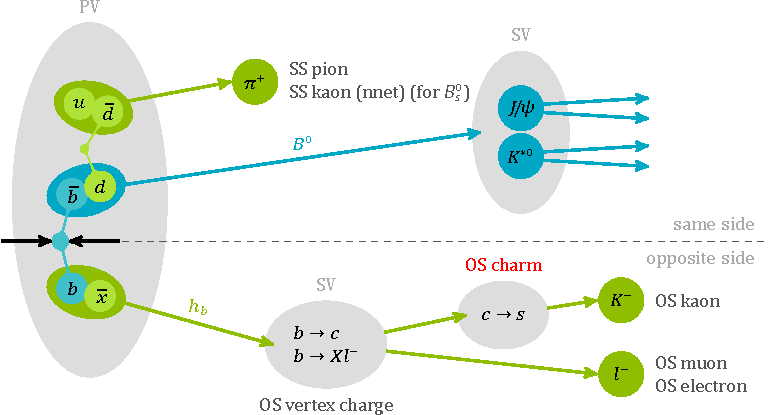
\includegraphics[width=0.68\textwidth, angle=0]{figs/FlavourTaggerScheme.pdf}
		\small{\caption{Scheme of the different flavour tagging algorithms. Same side taggers are shown in the upper part, opposite side taggers in the lower part.}}
		\label{fig:flavtagscheme}
	\end{center}
\end{figure}

\section{Flavour Tagging algorithms at LHCb}\label{sec:2}

For the opposite side tagging algorithms there are mainly two different types of algorithms. Single particle taggers identify electrons, muons and kaons coming from the other $b$ hadron. To select these particles a large impact parameter significance  with respect to the primary vertex and a large transverse momentum $p_\text{T}$ are required. For particle identification requirements on the difference between the logarithm of the likelihood for the muon, electron, kaon or proton and the pion hypothesis are applied. In case of multiple candidates from one tagging algorithm the candidate with the highest transverse momentum is chosen.\\
In contrast to this method the OS vertex charge tagger does not use single tracks but a weighted charge of a secondary vertex to take a tag decision. The secondary vertex is reconstructed from two tracks which have the highest probablity to originate from the OS $b$ hadron. From this seed more tracks that are compatible with coming from the secondary vertex but not from the primary vertex are added to the vertex to form the final $b$hadron candidate. Finally a weighted charge is calculated as a sum of the charges $Q_i$ of all tracks associated to the vertex
\begin{equation}
Q_\text{vtx}=\frac{\sum_i p_T^k(i)Q_i}{\sum_i p_T^k(i)},
\end{equation} 
weighted by their transverse momentum $p_T$ to the power $k$. The value $k$ optimises the effective tagging efficiency.\\
For the same side tagging one has to distinguish between $B_d^0$ and $B_s^0$ mesons as the accompanying quark is a $d$ or a $s$ quark, respectively. In case of a $B_d^0$ meson an additional charged pion from the $d$ quark, which can hadronise with an $u$ quark, emerges. Also pions from excited states as $B^*$ and $B^{**}$ have the same charge as pions from the direct fragmenation process with a $B^0$ meson. Therefore the pion candidates are required to be charged particles with high momentum and transverse momentum originating from the primary vertex \cite{10}. If the signal $B$ meson is a $B_s^0$, a kaon can be formed from the additional $s$ quark and an $u$ quark.\\

\subsection{SS kaon tagging using neural nets (NN)}

The first version of the SS kaon tagger developed at the LHCb experiment uses a selection based on a sequential set of requirements on some discriminating variables to identify the tagging kaon and a neural net (NN) to estimate the mistag probabilty $\eta$. An updated version of this tagger, the SS kaon neural net tagger, uses two NN. The first NN distinguishes between fragmentation tracks and the underlying event tracks (see figure \ref{fig:nnet}). The fragmentation tracks are the signal tracks for the SS kaon tagger, i.e. the tracks are the searched tagging particle tracks \cite{2}. 
\begin{figure}[htbp]
	\begin{center}
		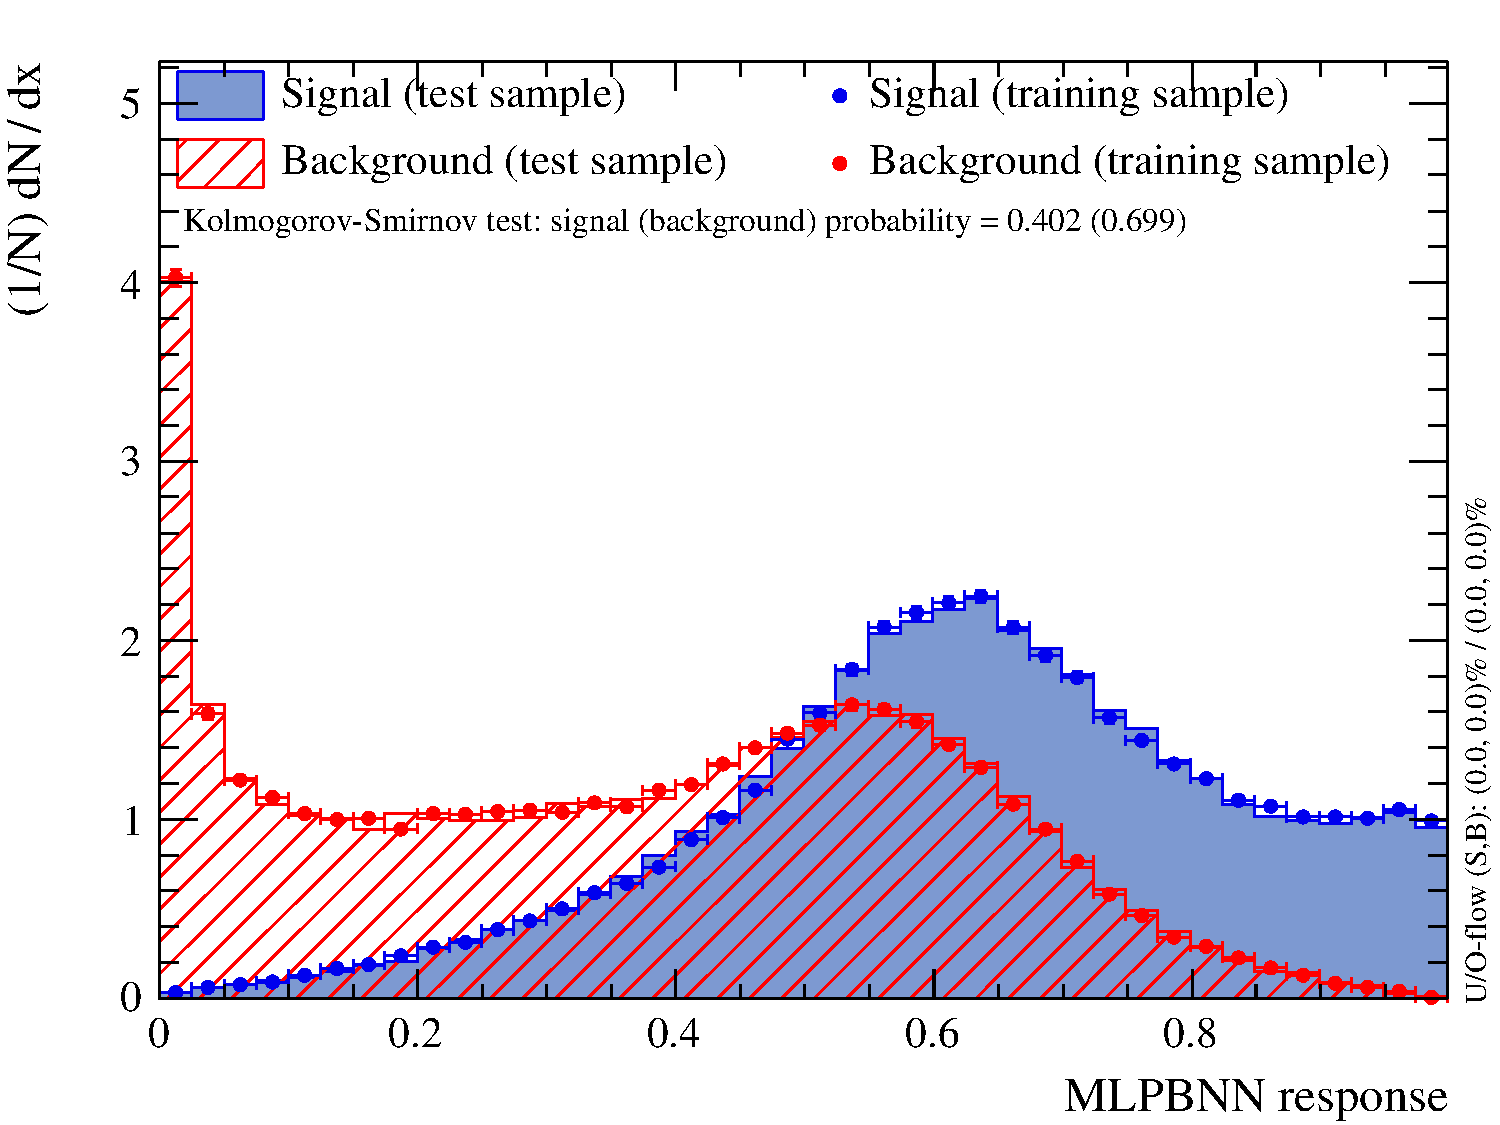
\includegraphics[width=0.58\textwidth, angle=0]{figs/sskaonNnetfirstNN3.pdf}
		\small{\caption{Distribution of NN response for fragmentation tracks (signal) and underlying event tracks (background) \cite{2}}}
		\label{fig:nnet}
	\end{center}
\end{figure}
The second NN assigns the final tag and mistag \cite{13}.\\ 
Compared to the \enquote{cut-based} SS kaon, the SS kaon NN gives a relative improvement of \SI{50}{\%} (\SI{41}{\%}) in $\varepsilon_\text{eff}$ for $B_s^0\to D_s^-\pi^+$ ($B_s^0\to J\!/\!\psi\phi$). This improvements can be observed also when comparing the effective tagging efficiencies in the measurements of $\phi_s$ at LHCb. The effective tagging efficiencies $\varepsilon_\text{eff}$ for the $C\!P$ analyses in \mbox{$B_s^0\to J\!/\!\psi K^+K^-$}, $\bar{B}_s^0\to J\!/\!\psi \pi^+\pi^-$ and $\bar{B}_s^0\to D_s^+D_s^-$ are listed in table \ref{tab:phis}.
\small \begin{table}[htbp]
  \centering
  \begin{tabular}{lcc}
  \toprule
	Decay mode & $\varepsilon_\text{eff}$ (\SI{1}{fb^{-1}}) & $\varepsilon_\text{eff}$ (\SI{3}{fb^{-1}}) \\
  \midrule
	$B_s^0\to J\!/\!\psi K^+K^-$ & \SI{3.13}{\%} \cite{3} & \SI{3.73}{\%} \cite{4} \\ 
	$\bar{B}_s^0\to J\!/\!\psi \pi^+\pi^-$ & \SI{2.43}{\%} \cite{5} & \SI{3.89}{\%} \cite{6} \\
	$\bar{B}_s^0\to D_s^+D_s^-$ & - & \SI{5.33}{\%} \cite{7} \\
  \bottomrule
  \end{tabular}
 \small{ \caption{Effective tagging efficiencies of the combination of the OS taggers and the SS kaon tagger for the $C\!P$ analyses measuring $\phi_s$. In the analyses on \SI{1}{fb^{-1}} the cut-based version of the SS kaon was used, the analyses on the whole Run I dataset with \SI{3}{fb^{-1}} used the neural net based version. }}
  \label{tab:phis}
\end{table} 
\normalsize
\subsection{OS charm tagger}

A novel tagger introduced at the end of Run I is the OS charm tagger. It uses charm hadrons from the decay chain $b\to c$ from the opposite side $b$ quark to tag the initial flavour. The reconstructed $D$ modes related to the OS $b$ decay are listed in table \ref{tab:OScharm}.
\small\begin{table}[htbp]
  \centering
  \begin{tabular}{lrr}
  \toprule
  Decay mode &Relative $\varepsilon_\text{tag}$ & Relative $\varepsilon_\text{eff}$ \\
  \midrule
  $D^0\to K^-\pi^+$ & \SI{10.0}{\%} & \SI{24.0}{\%} \\ 
  $D^0\to K^-\pi^+\pi^+\pi^-$ & \SI{5.9}{\%} & \SI{8.4}{\%} \\
  $D^+\to K^-\pi^+\pi^+$ & \SI{10.3}{\%} & \SI{2.6}{\%} \\
  $D^0,D^+\to K^-\pi^+X$ & \SI{69.7}{\%} & \SI{61.5}{\%} \\
  $D^0,D^+\to K^-e^+X$ & \SI{0.5}{\%} & \SI{0.2}{\%} \\
  $D^0,D^+\to K^-\mu^+X$ & \SI{3.4}{\%} & \SI{0.3}{\%} \\
  $\Lambda_c^+\to p^+K^-\pi^+$ & \SI{0.2}{\%} & \SI{2.4}{\%} \\
  \bottomrule
  \end{tabular}
  \small{\caption{$D$ meson decay modes with their relative contributions to $\varepsilon_\text{tag}$ and $\varepsilon_\text{eff}$ which are used by the OS charm tagger.}}
  \label{tab:OScharm}
\end{table}\normalsize
For each mode one boosted decision tree is used to calculate the mistag probybility $\eta$ and then the candidate with the best prediction is picked \cite{12}. The OS charm tagger provides a relatively clean measure of the $B$ flavour, i.e. it provides low values of $\eta$. Depending on the decay mode its stand-alone effective tagging efficiency is between \SI{0.30}{\%} and \SI{0.40}{\%} \cite{12}.

\section{Calibration of the Flavour Tagging}\label{sec:3}

The mistag estimate $\eta$ provided by the different tagging algorithms has to be corrected and transformed into the true mistag probabilty $\omega$. This is done with a linear calibration function
\begin{equation}
\omega(\eta)=p_0+p_1\left(\eta-\langle\eta\rangle\right)\label{eq:linfunc}
\end{equation}
where $\langle\eta\rangle$ is the mean mistag estimate. The parameters $p_0$ and $p_1$ of this calibration function are extracted in to different ways. Using charged decay modes as $B^+\to J\!/\!\psi K^+$ and $B^+\to D^0\pi^+$ the true mistag $\omega$ can be extracted by comparing the tag decision with the charge of the kaon or pion in the final state. In neutral decay modes as $B^0\to J\!/\!\psi K^{*0}$, $B^0\to D^{*-}\mu^+\nu_\mu$ or $B_s^0\to D_s^-\pi^+$ a full time-dependent analysis is needed to extract omega from the mixing asymmetry:
\begin{equation}
A_\text{mix}(t)\propto\left(1-2\omega\right)\cos\left(\Delta m_{d/s} t\right)\label{eq:mix}
\end{equation}
In both cases the calculation of $\omega$ is done in bins of the mistag estimate $\eta$ and the linear function \ref{eq:linfunc} is fitted to the $(\omega,\eta)$ pairs. Figure \ref{fig:calibration} shows the time dependent mixing asymmetry of equation \ref{eq:mix} in the case of the $B^0\to J\!/\!\psi K^{*0}$ decay and the linear calibration function resulting from the fit of all the bins in $\eta$.\\ 
\begin{figure}[htbp]
	\begin{center}
		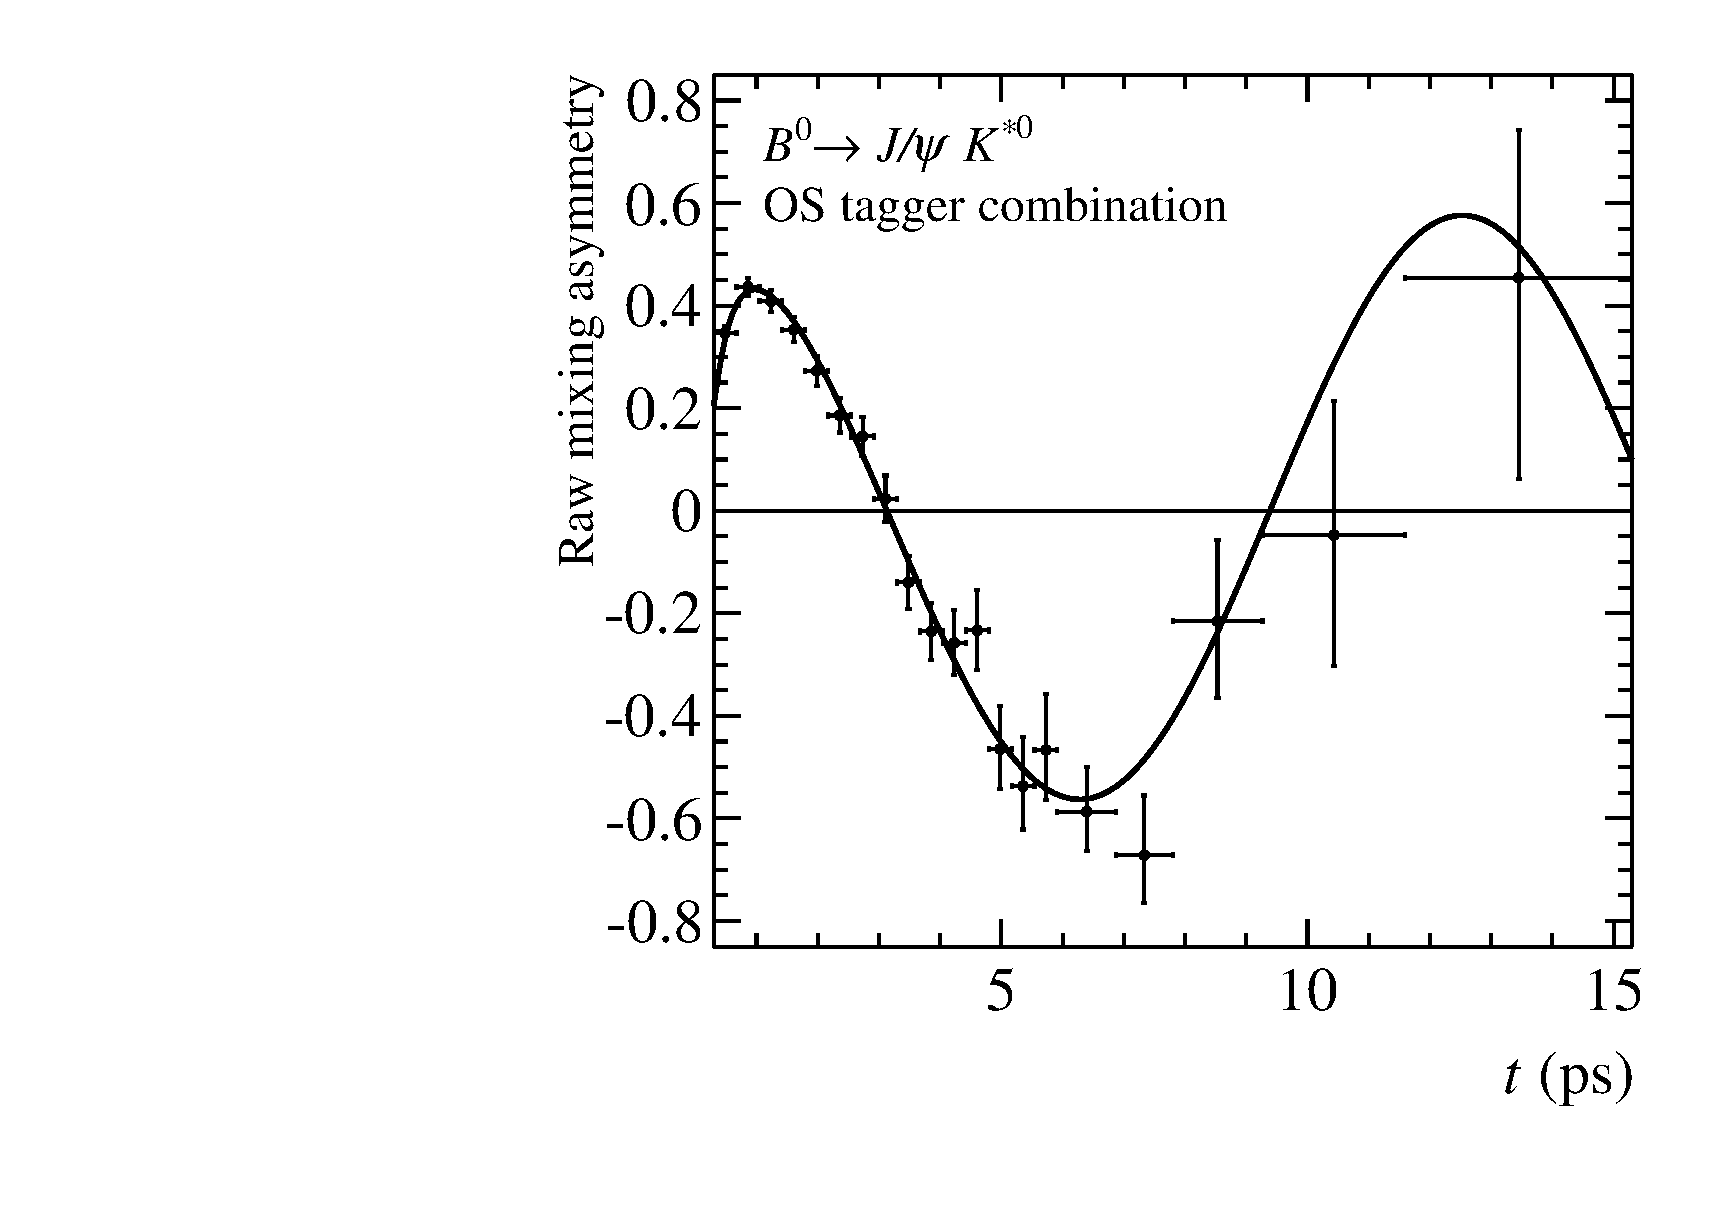
\includegraphics[width=0.34\textwidth, angle=0]{figs/KstAsym.pdf}
		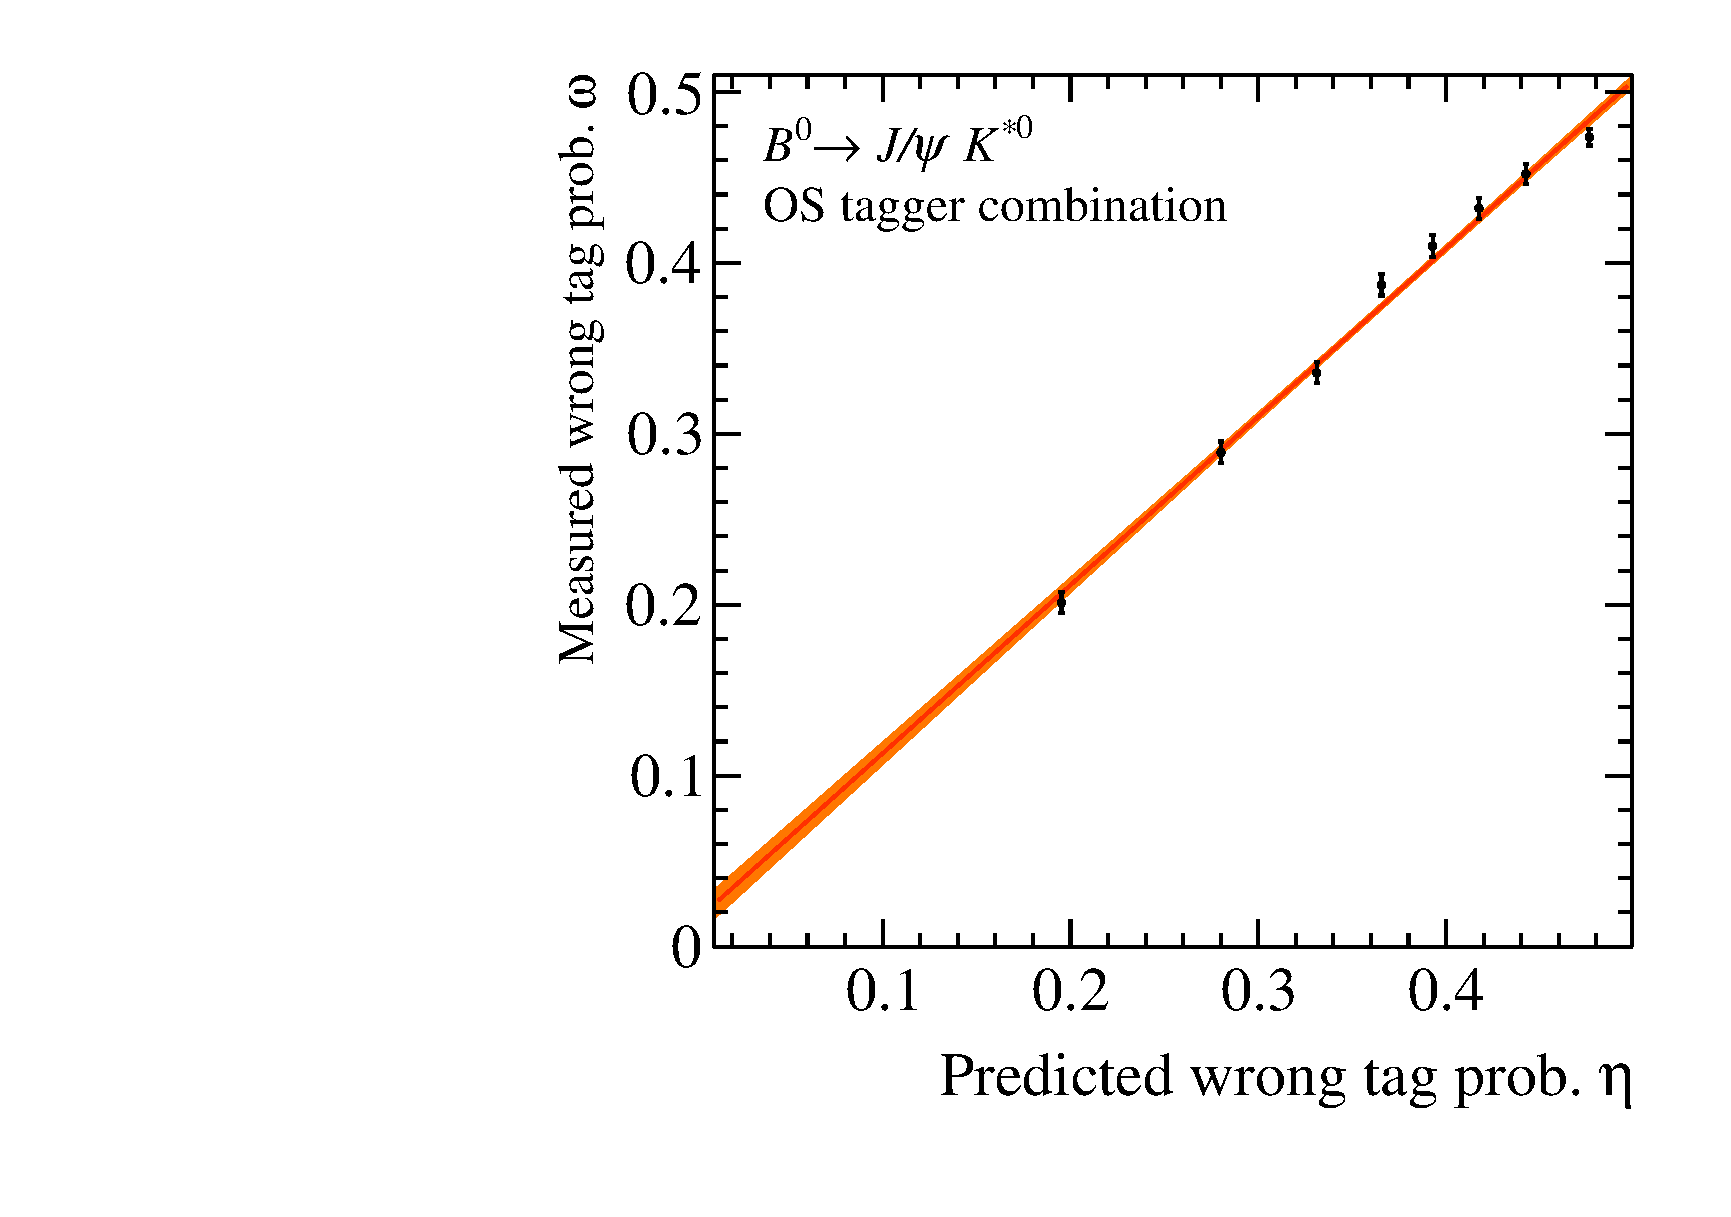
\includegraphics[width=0.34\textwidth, angle=0]{figs/Bd2JpsiKst-Kst-OST-8ScalingFunction_raw.pdf}
		\small{\caption{Overall mixing asymmetry (left) and resulting calibration function (right) for the OS tagger combination in the calibration mode $B^0\to J\!/\!\psi K^{*0}$.}}
		\label{fig:calibration}
	\end{center}
\end{figure}
In time-dependent analyses of neutral $b$ mesons, systematic uncertainties coming from the Flavour Tagging are assigned for the uncertainties associated with the calibration method and for the portability of the calibration from the control to the signal decay mode. Adding these two categories of systematic uncertainties, the size of the systematic uncertainty is of the order of the size of the statistical uncertainty on the calibration.
For most analyses  during Run I the systematic uncertainties are much smaller than the statistical uncertainties. Therefore one calibration per tagger valid for all channels is provided.\\
For analyses where the systematic uncertainties are dominated by the Flavour Tagging uncertainties and the systematic uncertainties are of the order of the statistical uncertainties an \enquote{ad-hoc} calibration using the best-suited control channel for the analyses is performed.

\subsection{$\bm{C\!P}$ violation in $\bm{B^0}\bm{\to} \bm{J\!/\!\psi K_s^0}$ $\pmb{(\sin 2\beta)}$}

The measurement of $C\!P$ violation in $B^0\to J\!/\!\psi K_s^0$ was performed on \SI{1}{fb^{-1}} and updated using the whole Run I dataset of \SI{3}{fb^{-1}}. The effective tagging power increased from $\varepsilon=\SI{2.38}{\%}$ (\SI{1}{fb^{-1}}) \cite{9} to $\varepsilon=\SI{3.02}{\%}$ (\SI{3}{fb^{-1}}) \cite{10}. This increase was mainly due to the use of the SS pion tagger which adds more than \SI{0.376}{\%} in the newest analysis. As in the measurement of $\sin 2\beta$ the statistical uncertainties are of the order of the systematic uncertainties and the flavour tagging contribution was expected to be a dominant factor an \enquote{ad-hoc} calibration was performed. The OS taggers were calibrated with the control channel $B^+\to J\!/\!\psi K^+$, the SS pion tagger was calibrated with $B^0\to J\!/\!\psi K^{*0}$. For both decay modes the decay and kinematic properties of the tagging particles should be similar to the signal decay, especially as both are reconstructed in the $J\!/\!\psi X$ mode. Systematic uncertainties were evaluated on the calibration method itself and due to the portability to the \mbox{$B^0\to J\!/\!\psi K_s^0$} decay. This approach decreased the size of the systematic uncertainty coming from the flavour tagging calibration to \SI{33}{\%} of the total systematic uncertainty \cite{10}.

\begingroup
\setstretch{0.8}
\begin{thebibliography}{99}
\small\bibitem{1}LHCb Collaboration, R.Aaij et. al., {\it Opposite-side flavour tagging of $B$ mesons at the LHCb experiment, Eur.Phys.J.} C72 (2012) 2022
\small\bibitem{2}LHCb Collaboration, R. Aaij et. al., {\it Optimization and calibration of the same-side kaon \mbox{tagging} algorithm using hadronic $B_s^0$ decays in 2011 data,} LHCb-CONF-2012-033
\small\bibitem{13} G. A. Krocker, {\it Development and calibration of a same side kaon tagging algorithm and measurement of the $B_s^0-\bar{B_s^0}$ oscillation frequency $\Delta m_s$ at the LHCb experiment, } PhD thesis, Heidelberg U., Sep, 2013, CERN-THESIS-2013-213
\small\bibitem{3}LHCb Collaboration, R. Aaij et. al., {\it Measurement of $C\!P$ violation and the $B_s^0$ meson decay width difference with   $B_s^0\to J\!/\!\psi K^+K^-$ and \mbox{$\bar{B_s^0}\to J\!/\!\psi \pi^+\pi^-$} decays, } Phys.Rev. D87 (2013) 11, 112010
\small\bibitem{4}LHCb Collaboration, R. Aaij et. al., {\it Precision measurement of $C\!P$ violation in $B_s^0\to J\!/\!\psi K^+K^-$ decays, } Phys.Rev.Lett. 114 (2015) 4, 041801
\small\bibitem{5} LHCb Collaboration, R. Aaij et. al., {\it Measurement of the $C\!P$-violating phase $\phi_s$ in $\bar{B}_s^0\to J\!/\!\psi \pi^+\pi^-$ decays, } Phys.Lett. B713 (2012) 378-386
\small\bibitem{6} LHCb Collaboration, R. Aaij et. al., {\it Measurement of the $C\!P$-violating phase $\phi_s$ in $\bar{B}_s^0\to J\!/\!\psi \pi^+\pi^-$ decays, } Phys.Lett. B736 (2014) 186-195
\small\bibitem{7} LHCb Collaboration, R. Aaij et. al., {\it Measurement of the $C\!P$-violating phase $\phi_s$ in $\bar{B}_s^0\to D_s^+D_s^-$ decays, } Phys.Rev.Lett. 113 (2014) 21, 211801
\small\bibitem{12} LHCb Collaboration, R. Aaij et. al., {\it $B$ flavor tagging using reconstructed charm decays at the LHCb experiment, } LHCb-PAPER-2015.027
\bibitem{9} LHCb Collaboration, R. Aaij et. al., {\it Measurement of the time-dependent $C\!P$ asymmetry in $B^0\to J\!/\!\psi K_s^0$ decays, } Phys.Lett. B721 (2013) 24-31
\small\bibitem{10} LHCb Collaboration, R. Aaij et. al., {\it Measurement of $C\!P$ violation in \mbox{$B^0\to J\!/\!\psi K_s^0$} decays, } Phys.Rev.Lett. 115 (2015) 3, 031601


\end{thebibliography}
\endgroup 


\end{document}
